\chapter{Wprowadzenie}
\label{cha:wprowadzenie}

Przedstawiony raport ma na celu przetestowania aplikacji Moodle, wykorzystując do tego celu oprogramowanie do testowania W3AF.

%---------------------------------------------------------------------------

\section{Zawartość raportu}
\label{sec:zawartoscPracy}
Struktura raportu jest następująca: 
\begin{itemize}
\item W pierwszym rozdziale opisany został program W3AF, jego konfiguracja oraz użyte pluginy. 
\item W rozdziale drugim omówiona została testowana aplikacja 
\item W rozdziale trzecim prezentujemy testy jakie przeprowadziliśmy na wybranej przez nas aplikacji.
\item W rozdziale czwartym zawarto wnioski 
\end{itemize}

%---------------------------------------------------------------------------

\section{W3AF}
W3AF (Web application attack and audit framework) to aplikacja open-source służąca do testowania bezpieczeństwa aplikacji internetowych Projekt zapewnia skaner podatności oraz narzędzia służące do wydobywania informacji z aplikacji internetowych. Dostarcza niezbędnych informacji o podatnościach na ataki dla wykonania testów penetracyjnych. Aplikacja dostarcza interfejs graficzny do wykonywania testów. Dostępny jest również interfejst tekstowy z linii komend.
\\
W3AF jest podzielony na dwie główne części, rdzeń oraz pluginy. Rdzeń koordynuje prace wszystkich procesów oraz dostarcza featury dostępne dla pluginów, które znajdują podatności oraz wykorzystują je. Pluginy są połączone ze sobą oraz dzielą się informacjami, używając do tego wspólnej bazy wiedzy. Pluginy mogą być podzielone na:
\begin{itemize}
\item Discovery
\item Audit
\item Grep
\item Attack
\item Output
\item Evasion
\item Bruteforce
\end{itemize}

\section{Użyte pluginy}

Do przetestowania aplikacji użyliśmy profilu OWASP\_TOP10, który bada aplikację pod kątem podatności na 10 najczęściej występujacych zagrożeń. Pluginy, które są wykorzystane to:
\begin{itemize}
\item csrf
\item htaccess\_methods
\item webspider
\item blind\_sqli
\item sqli
\item xss
\item buffer\_overflow
\end{itemize}

\section{Konfiguracja}

Niestety na systemie operacyjnym OSX nie jest możliwa praca z W3AF w trybie graficznym. Powodem tego jest występowanie błędu podczas uruchomienia. Spowodowane jest to bugiem w jednej z bibliotek pythona używanych do grafiki. Cała konfiguracja została zatem wykonana za pomocą linii komend. Aby uruchomić W3AF w linii komend, należy uruchomić skrypt a3wf\_console. Po uruchomieniu konsoli i wypisaniu prompta można przystąpić do konfiguracji frameworku. Z poziomu lini komend możemy dowolnie konfigurować działanie programu. Możemy wybrać, które pluginy będą używane, możemy, a nawet musimy skonfigurować cel naszych ataków w opcji target.
\noindent
\begin{minipage}{\linewidth}
\makebox[\linewidth]{
  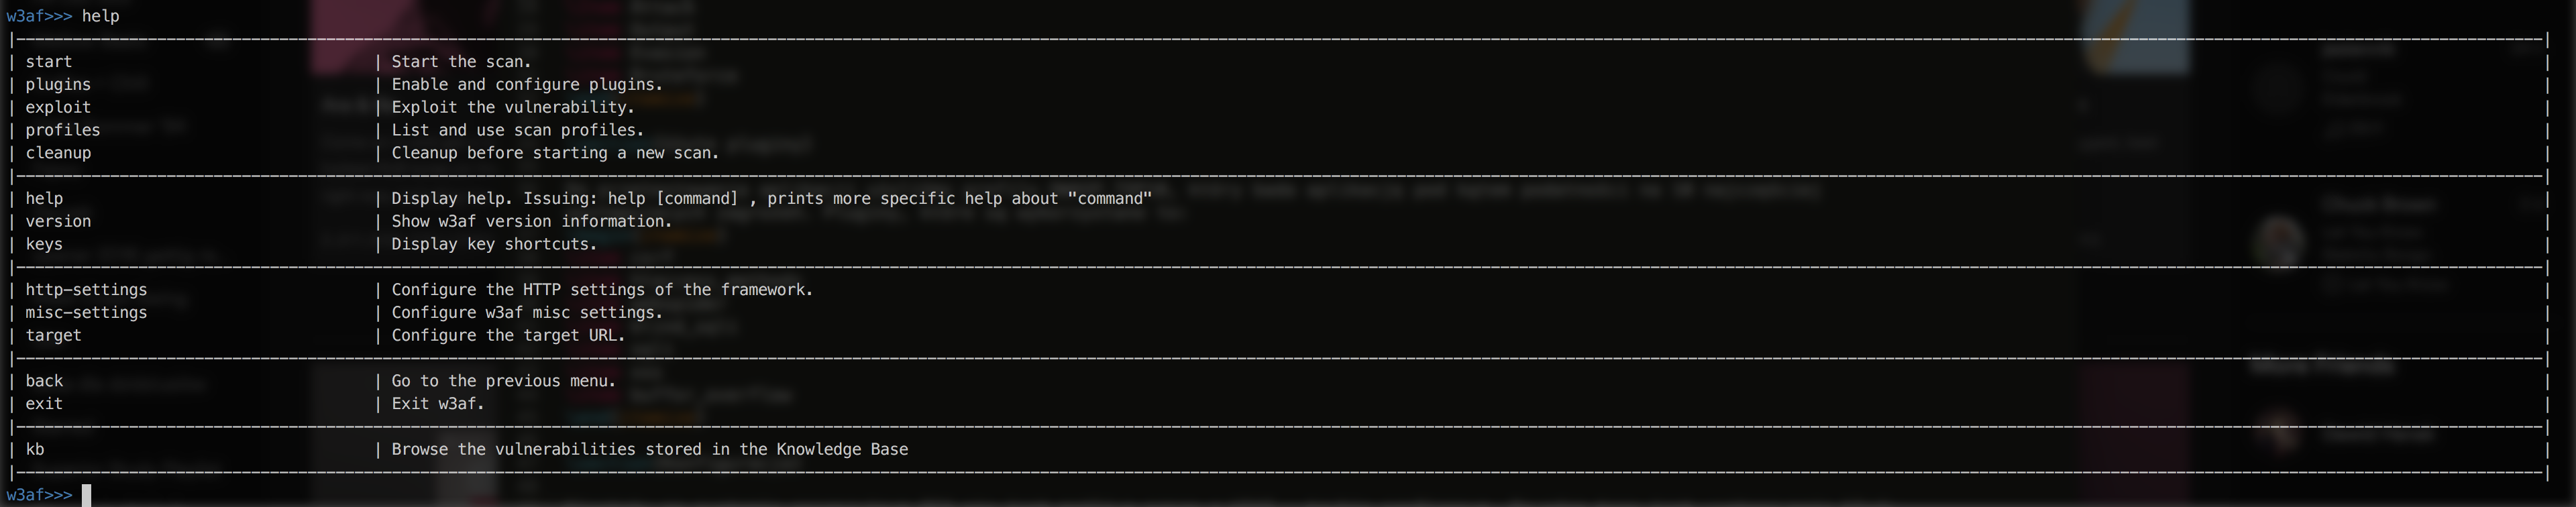
\includegraphics[keepaspectratio=true,scale=0.2]{pictures/options.png}}
\captionof{figure}{Opcje W3AF do wyboru}\label{erd}
\end{minipage}

\noindent
\begin{minipage}{\linewidth}
\makebox[\linewidth]{
  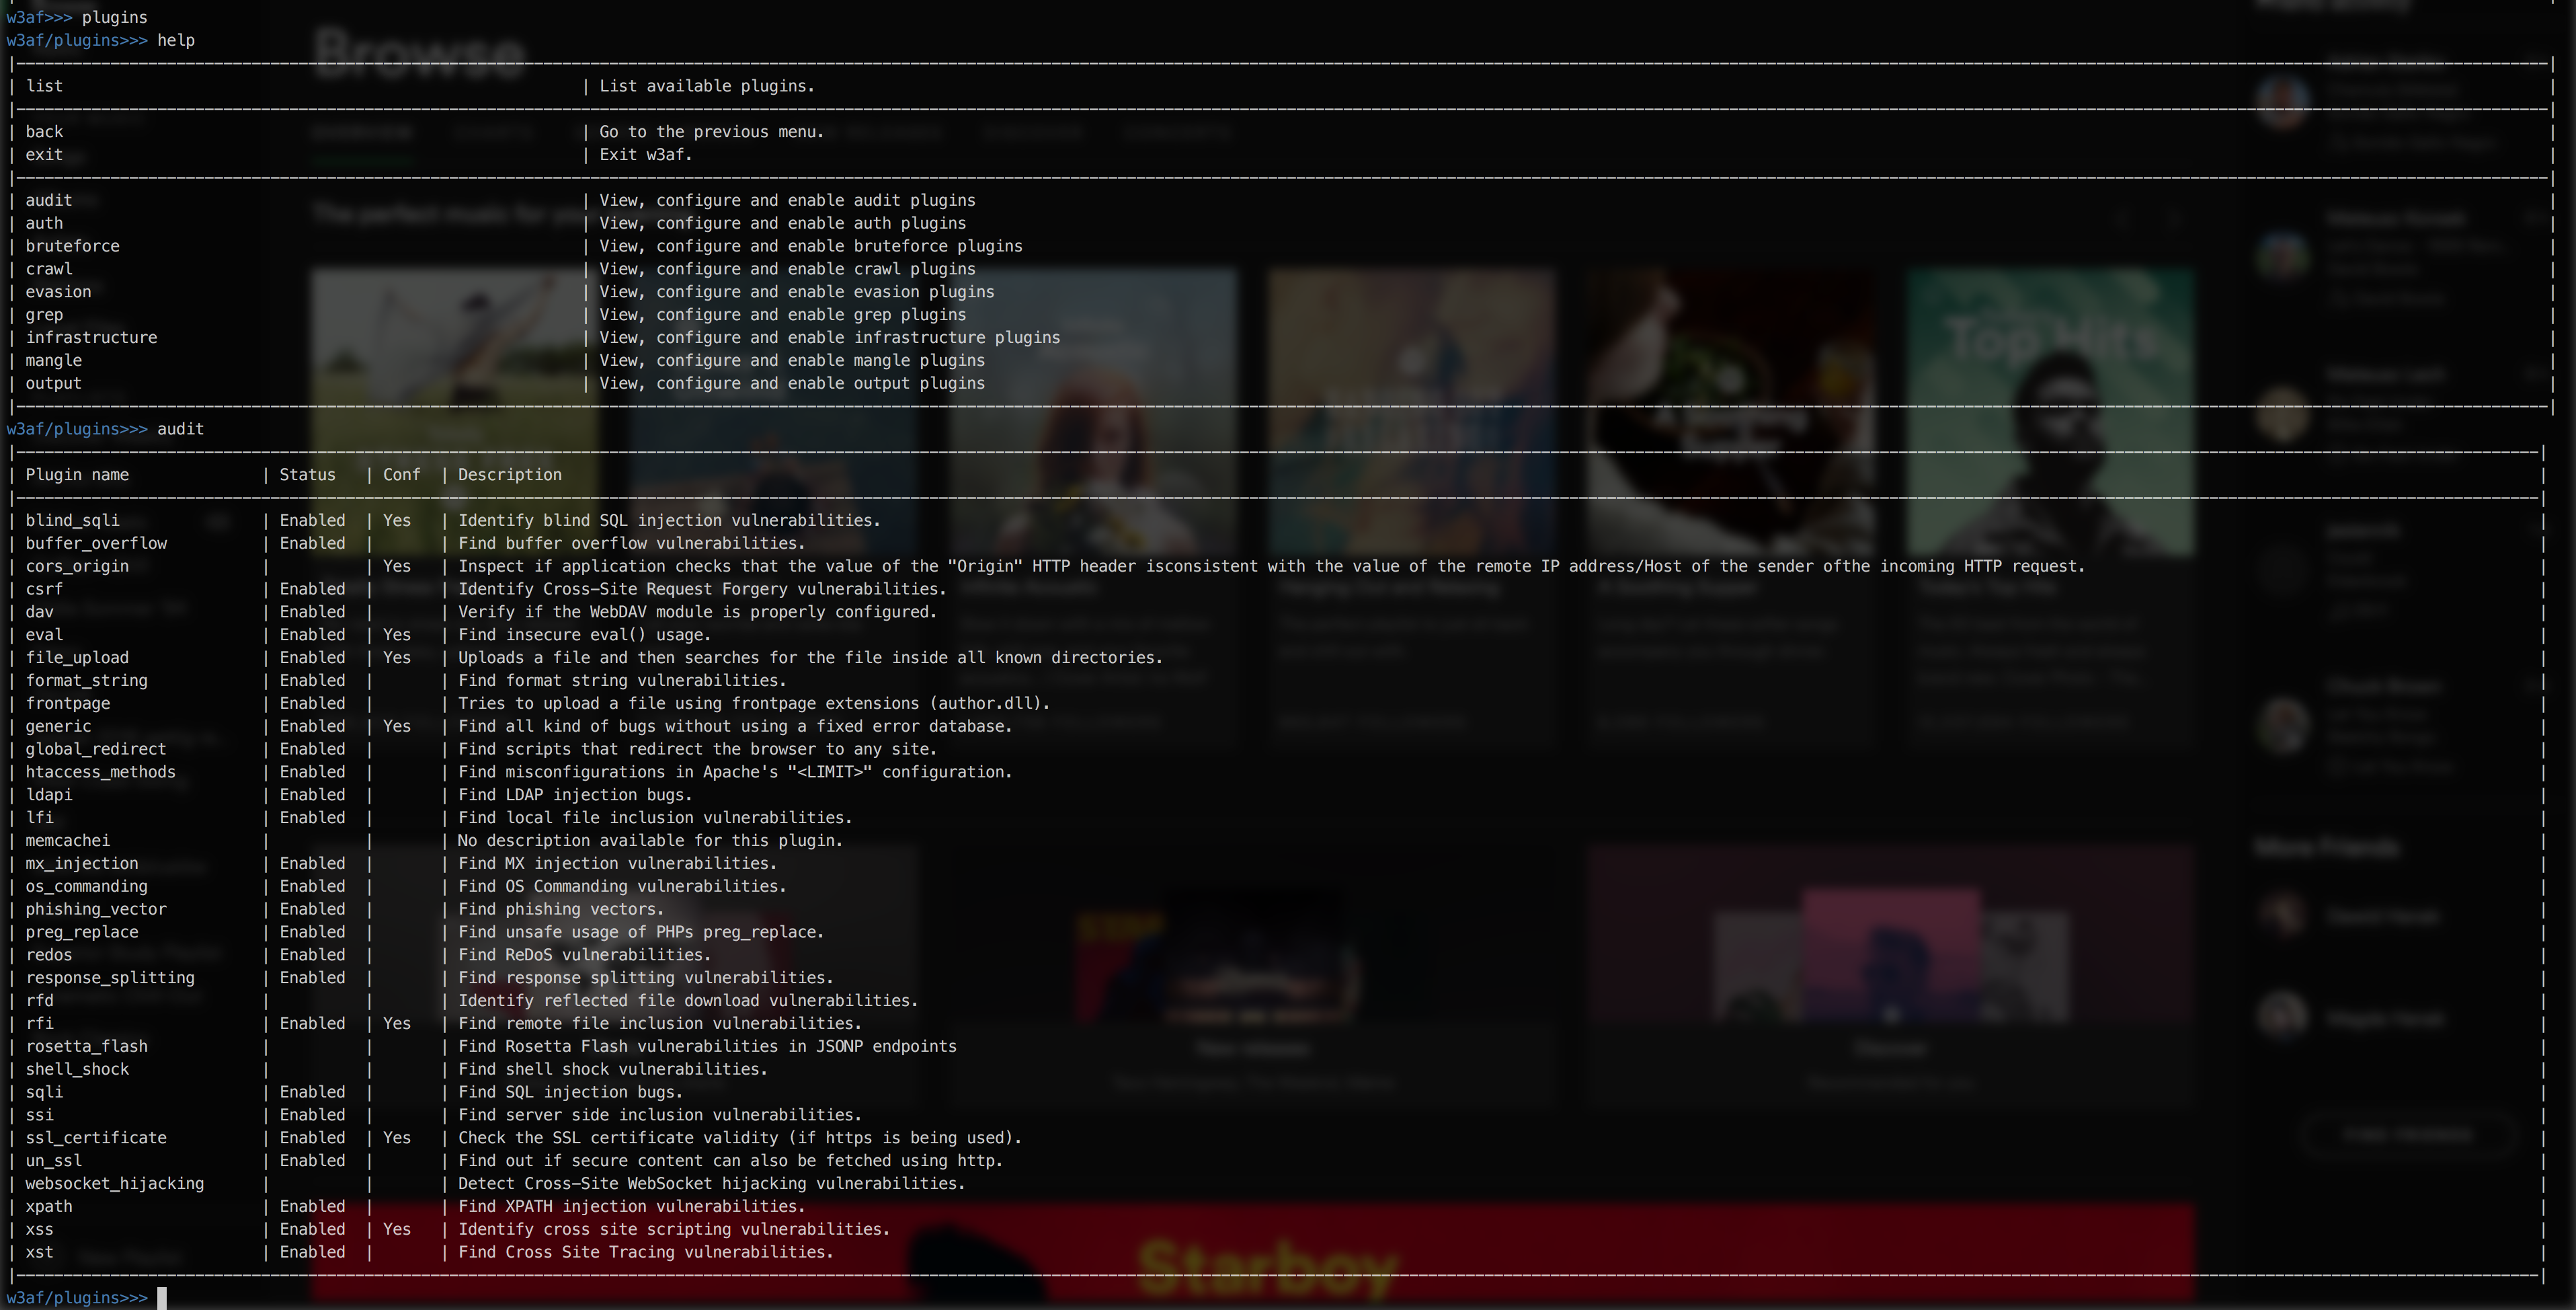
\includegraphics[keepaspectratio=true,scale=0.2]{pictures/plugins.png}}
\captionof{figure}{Różnorodność pluginów do wyboru}\label{erd}
\end{minipage}

\noindent
\begin{minipage}{\linewidth}
\makebox[\linewidth]{
  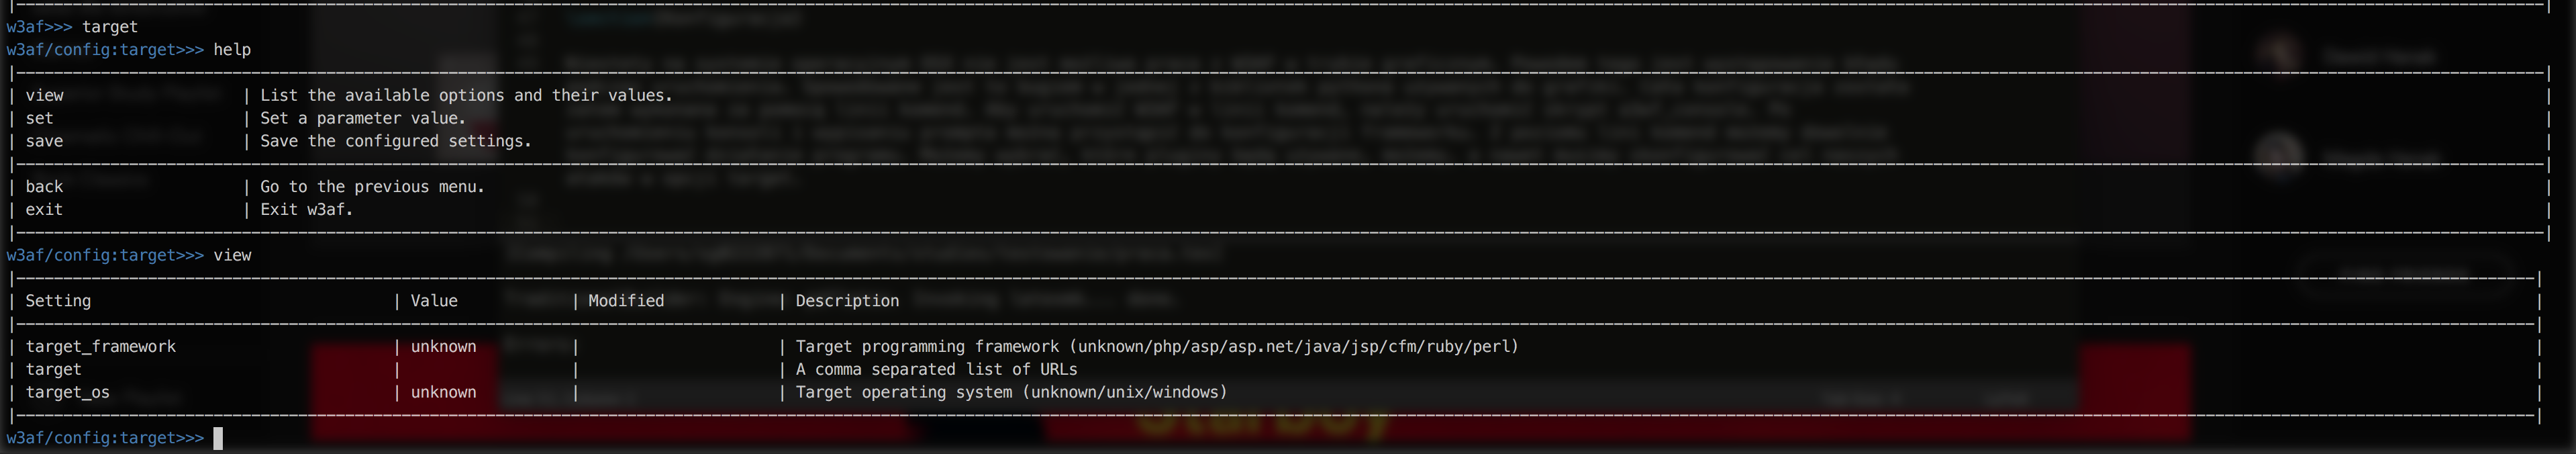
\includegraphics[keepaspectratio=true,scale=0.2]{pictures/target.png}}
\captionof{figure}{Konfiguracja celu ataków}\label{erd}
\end{minipage}

Ostatecznie główne testy przeprowadziliśmy wykorzystując tryb graficzny w3af na systemie Windows. W celu rozpoczęcia pracy należało ustawić URL docelowo testowanej aplikacji wraz z informacją na jakim systemie operacyjnym zostaną wykonane testy, a także technologię w jakiej napisany został testowany kod. Ustawienie tych elementów przedstawia poniższy zrzut:

\noindent
\begin{minipage}{\linewidth}
\makebox[\linewidth]{
  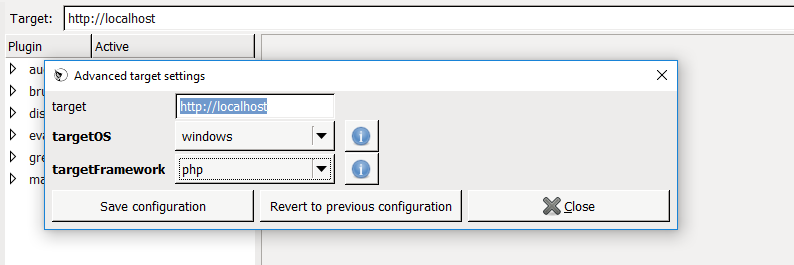
\includegraphics[keepaspectratio=true,scale=0.7]{pictures/w3afconf.png}}
\captionof{figure}{Konfiguracja w3af}\label{erd}
\end{minipage}
\end{enumerate}

W3af oferuje nam szereg różnego rodzaju testów wraz z gotowymi profilami do wyboru, które definiują określony sposób testowania aplikacji. Ten wachlarz możliwości widzimy na zrzucie:

\noindent
\begin{minipage}{\linewidth}
\makebox[\linewidth]{
  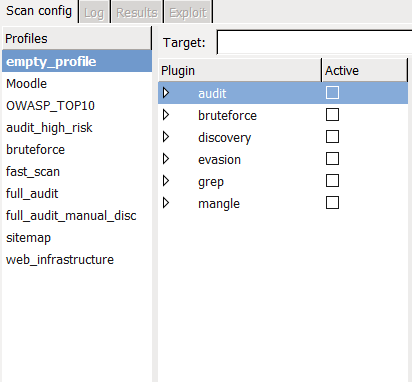
\includegraphics[keepaspectratio=true,scale=0.7]{pictures/w3aftests.png}}
\captionof{figure}{Profile oraz dostępne pluginy}\label{erd}
\end{minipage}
\end{enumerate}





